\documentclass[11pt,a4paper,fontset=fandol]{ctexart}
\usepackage[margin=2cm,top=1.7cm,bottom=1.8cm]{geometry}
\usepackage{amsmath,amssymb,mathtools}
\usepackage{tikz}
\usepackage{xcolor}
\usepackage{enumitem}
\usepackage{booktabs}
\usepackage{array}
\usepackage{fancyhdr}
\usepackage[user,lastpage]{zref}
\usepackage{tcolorbox}

\setlength{\parindent}{2em}
\setlength{\parskip}{0.4em}
\pagestyle{fancy}
\setlength{\headheight}{14pt}
\fancyhf{}
\fancyhead[L]{向量、函数与立体几何期末综合测试卷——教师版详细教案与解析}
\fancyfoot[C]{第 \thepage\ 页，共 \zpageref{LastPage} 页}
\renewcommand{\headrulewidth}{0.4pt}
\renewcommand{\footrulewidth}{0pt}

\newcommand{\vect}[1]{\overrightarrow{#1}}
\newcommand{\ans}[1]{\boxed{#1}}
\newcommand{\method}[1]{\par\medskip\noindent\textbf{解法 #1}\par}

\newtcolorbox{answerbox}{colback=gray!5,colframe=black!55,boxrule=0.6pt,arc=1mm,left=8pt,right=8pt,top=6pt,bottom=6pt}
\newtcolorbox{problembox}{colback=blue!2!white,colframe=blue!40!black,boxrule=0.6pt,arc=1.5mm,left=8pt,right=8pt,top=6pt,bottom=6pt}
\newtcolorbox{note}{colback=orange!5!white,colframe=orange!80!black,boxrule=0.5pt,arc=1mm,left=8pt,right=8pt,top=6pt,bottom=6pt}

\definecolor{ink}{RGB}{35,35,35}
\definecolor{gold}{RGB}{218,165,32}
\tikzset{
  geom/.style={thick,draw=blue!80!black},
  aid/.style={thin,draw=gray!60},
  hline/.style={thick,draw=gold!90!black},
  vline/.style={thick,draw=teal,->,>=stealth},
  vpoint/.style={circle,fill=black,inner sep=1.2pt},
  centerpt/.style={circle,fill=gray!80,inner sep=1.2pt},
  moving/.style={circle,fill=gold!90!black,inner sep=1.5pt}
}

% TikZ Figures
\newcommand{\figCone}{%
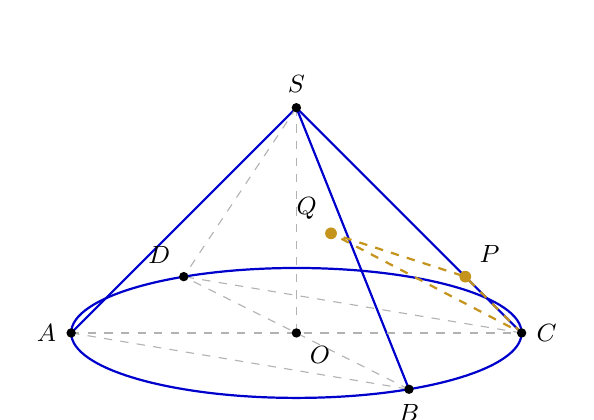
\begin{tikzpicture}[scale=1.1,every node/.style={font=\small}]
  \draw[geom] (0,0) ellipse (2.6cm and 0.75cm);
  \coordinate (O) at (0,0);
  \coordinate (S) at (0,2.6);
  \coordinate (A) at (-2.6,0);
  \coordinate (C) at (2.6,0);
  \coordinate (D) at (-1.3,0.65);
  \coordinate (B) at (1.3,-0.65);
  \coordinate (P) at (1.95,0.65);
  \coordinate (Q) at (0.4,1.15);
  
  \draw[geom] (S)--(A);
  \draw[geom] (S)--(C);
  \draw[geom] (S)--(B);
  \draw[aid,dashed] (S)--(D);
  \draw[aid,dashed] (S)--(O);
  \draw[aid,dashed] (A)--(C);
  \draw[aid,dashed] (B)--(D);
  \draw[aid,dashed] (A)--(B);
  \draw[aid,dashed] (C)--(D);
  \draw[hline,draw=gold!90!black,thick,dashed] (C)--(P)--(Q)--cycle;
  
  \node[vpoint,label=above:$S$] at (S){};
  \node[vpoint,label=below right:$O$] at (O){};
  \node[vpoint,label=left:$A$] at (A){};
  \node[vpoint,label=right:$C$] at (C){};
  \node[vpoint,label=below:$B$] at (B){};
  \node[vpoint,label=above left:$D$] at (D){};
  \node[moving,label=above right:$P$] at (P){};
  \node[moving,label=above left:$Q$] at (Q){};
\end{tikzpicture}}

\newcommand{\figGeneralCentroid}{%
\begin{tikzpicture}[scale=1.05,every node/.style={font=\small}]
  \coordinate (A) at (0.5, 3.0);
  \coordinate (B) at (-2.0, 0);
  \coordinate (C) at (2.5, 0);
  \coordinate (G) at (0.333, 1.0);
  \coordinate (D) at (-1.0, 1.2);
  \coordinate (E) at (2.0, 0.75);
  
  \draw[geom] (A)--(B)--(C)--cycle;
  \draw[aid,dashed] (A)--(0.25,0);
  \draw[hline,draw=gold!90!black,thick] (-1.6, 1.29)--(2.4, 0.69) node[right,font=\scriptsize,text=gold!90!black] {直线 \(l\)};
  
  \node[vpoint,label=above:$A$] at (A){};
  \node[vpoint,label=below left:$B$] at (B){};
  \node[vpoint,label=below right:$C$] at (C){};
  \node[centerpt,label=below left:$G$] at (G){};
  \node[moving,label=above left:$D$] at (D){};
  \node[moving,label=above right:$E$] at (E){};
\end{tikzpicture}}

\newcommand{\figIsogonalTriangle}{%
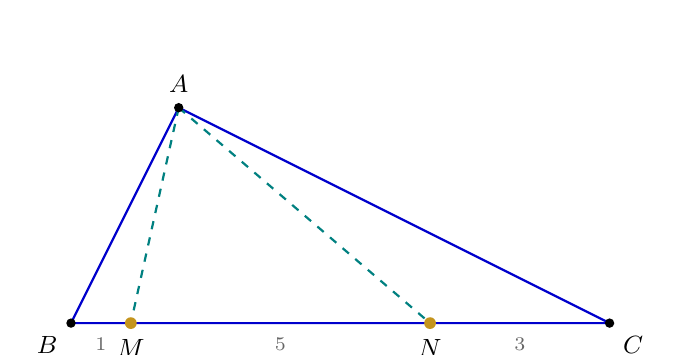
\begin{tikzpicture}[scale=0.95,every node/.style={font=\small}]
  \coordinate (B) at (0,0);
  \coordinate (M) at (0.8,0);
  \coordinate (N) at (4.8,0);
  \coordinate (C) at (7.2,0);
  \coordinate (A) at (1.44,2.88);
  
  \draw[geom] (A)--(B)--(C)--cycle;
  \draw[aid,dashed,thick,draw=teal] (A)--(M);
  \draw[aid,dashed,thick,draw=teal] (A)--(N);
  
  \node[vpoint,label=above:$A$] at (A){};
  \node[vpoint,label=below left:$B$] at (B){};
  \node[moving,label=below:$M$] at (M){};
  \node[moving,label=below:$N$] at (N){};
  \node[vpoint,label=below right:$C$] at (C){};
  
  \path (B) -- (M) node[midway,below=2pt,font=\scriptsize,text=gray!80!black] {$1$};
  \path (M) -- (N) node[midway,below=2pt,font=\scriptsize,text=gray!80!black] {$5$};
  \path (N) -- (C) node[midway,below=2pt,font=\scriptsize,text=gray!80!black] {$3$};
\end{tikzpicture}}

\begin{document}

\begin{center}
{\Large\bfseries 向量、函数与立体几何期末综合测试卷}\\[0.4em]
{\Large\bfseries 教师版详细教案与全套解答（含原题与多解分析）}
\end{center}

\begin{answerbox}
\textbf{全卷答案速查表：}
\begin{center}
\begin{tabular}{c|cccccc|cc}
\toprule
题号 & 1 & 2 & 3 & 4 & 5 & 6 & 附加1 (7) & 附加2 (8)\\
\midrule
结论 & A & A & C & $[\frac{\sqrt3}{2},1]$ & 见详解 & 见详解 & A & $\frac12$\\
\bottomrule
\end{tabular}
\end{center}
\textbf{核心得分要点提示：}
\begin{enumerate}[leftmargin=1.5em,label=\arabic*.]
  \item 第 5 题圆锥题：两平面夹角余弦为 $\dfrac{1}{3}$，周长最小值为 $3\sqrt{2}$；
  \item 第 6 题重心题：三问结论依次为 $\dfrac{1}{\lambda}+\dfrac{1}{\mu}=3$、$\left[\dfrac{4}{9},\dfrac{1}{2}\right)$、$\dfrac{1}{3}$；
  \item 附加题区：第 7 题为充分不必要条件（选 A），第 8 题边长比为 $\dfrac{1}{2}$。
\end{enumerate}
\end{answerbox}

\vspace{1em}

\section*{一、 必答选择题解析（共 30 分）}

\subsection*{第 1 题（10 分）}

\begin{problembox}
已知定义在 \(\mathbb{R}\) 上的奇函数 \(f(x)\) 满足 \(f(x) = f(x - 6)\)，且当 \(0 \le x \le 3\) 时，
\[
f(x) = \begin{cases} 
a + \log_{0.5}(x + 1), & 0 \le x \le 1,\\[0.3em]
(x - 2)(x - 3), & 1 < x \le 3
\end{cases} \quad (a \text{ 为常数})
\]
则 \(f(2010) + f(2011) + \cdots + f(2026)\) 的值为（\qquad）\\[0.4em]
A. \(-1\) \qquad\qquad\qquad B. \(0\) \qquad\qquad\qquad C. \(1\) \qquad\qquad\qquad D. \(-2\)
\end{problembox}

\medskip
\begin{tcolorbox}[colback=gray!4,colframe=ink!70,boxrule=0.7pt,arc=1mm,before skip=6pt,after skip=6pt,top=4pt,bottom=4pt,title=\textbf{决策路线}]
\begin{enumerate}[label=\textbf{\arabic*\ },leftmargin=1.8em]
  \item \textbf{[目标定位]}：求有限序列和 \(\sum_{k=2010}^{2026} f(k)\)（共 17 项），目标状态为借助周期性及单周期内整数自变量的函数值和与余项和完成求值。
  \item \textbf{[约束扫描]}：定义域为 \(\mathbb{R}\)，奇函数 \(f(0)=0\)；周期约束：由 \(f(x)=f(x-6)\)，知 6 是函数 \(f\) 的一个周期；分段区间 \(0 \le x \le 3\)。
  \item \textbf{[表征选择]}：选择\textbf{周期离散序列表征}。将连续函数求和转化为“按模 6 余数分组的周期抵消”。
  \item \textbf{[路径检索]}：先利用 \(f(0)=0\) 求未知数 \(a\)；再依次求出 \(0,1,2,3,4,5\) 的函数值，计算单周期和 \(\sum_{k=0}^{5} f(k)\)。
  \item \textbf{[模型转化]}：项数统计 \(2026 - 2010 + 1 = 17\) 项。按模 6 分组：\(17 = 2 \times 6 + 5\)，转化为“2 个完整周期（和为 0）+ 前 5 个余项”。
  \item \textbf{[逻辑校验]}：将 \(2010 \sim 2021\) 分成两个完整周期，剩余 \(2022 \sim 2026\) 五项，对应模 6 余数 \((0,1,2,3,4)\)，求和得 \(0 + (-1) + 0 + 0 + 0 = -1\)。
  \item \textbf{[得分闭环]}：首项 \(2010 \equiv 0 \pmod 6\)，余项无漏项，最终答案确定为 \(-1\)。
\end{enumerate}
\end{tcolorbox}

\method{一：单周期项和计算法（推荐板书）}

\noindent\textbf{【触发信号】}
\begin{itemize}[leftmargin=1.5em]
  \item \textbf{如何想到求 $a=0$？} 看到“定义在 \(\mathbb{R}\) 上的奇函数”，首先检查自变量原点 \(f(0)=0\)。代入 \(0 \le x \le 1\) 段得到 \(a + \log_{0.5}(1) = 0 \implies a=0\)。
  \item \textbf{如何想到按模 6 分组？} 由关系式 \(f(x) = f(x-6)\)，可知 6 是函数 \(f\) 的一个周期。对于超大项数求和（如 2010 到 2026），逐项硬算容易繁琐，最自然的方式是将庞大项数“除以周期取余数”，将 17 项压缩为 5 项。
\end{itemize}

1. \textbf{求常数 $a$：}
由于 $f(x)$ 是定义在 $\mathbb{R}$ 上的奇函数，必有 $f(0) = 0$。
代入 $0 \le x \le 1$ 段的解析式：
\[
f(0) = a + \log_{0.5}(0 + 1) = a + 0 = a \implies a = 0.
\]

2. \textbf{计算一个周期内 6 个整数自变量的函数值：}
由分段解析式与奇偶性 $f(-x) = -f(x)$ 依次求值：
\begin{align*}
f(0) &= 0,\\[0.3em]
f(1) &= \log_{0.5}(1 + 1) = \log_{0.5} 2 = -1,\\[0.3em]
f(2) &= (2 - 2)(2 - 3) = 0,\\[0.3em]
f(3) &= (3 - 2)(3 - 3) = 0,\\[0.3em]
f(4) &= f(-2) = -f(2) = -0 = 0,\\[0.3em]
f(5) &= f(-1) = -f(1) = -(-1) = 1.
\end{align*}
因此，在任意连续 6 个整数项构成的完整周期中，函数值之和为：
\[
\sum_{k=0}^{5} f(k) = f(0) + f(1) + f(2) + f(3) + f(4) + f(5) = 0 + (-1) + 0 + 0 + 0 + 1 = \mathbf{0}.
\]

3. \textbf{项数统计与周期分组：}
求和式共有项数：
\[
N = 2026 - 2010 + 1 = 17 \text{ 项}.
\]
因为首项 $2010 = 6 \times 335 \equiv 0 \pmod 6$，故从 $2010$ 到 $2026$ 的余数分布恰好为：
\[
17 \text{ 项} = \underbrace{2 \text{ 个完整周期 (共 12 项，和为 0)}}_{2010 \sim 2021} + \underbrace{5 \text{ 个余项 (对应余数 0, 1, 2, 3, 4)}}_{2022 \sim 2026}.
\]

4. \textbf{计算余项之和：}
余下的最后 5 项分别对应模 6 余数 $0, 1, 2, 3, 4$：
\begin{align*}
f(2022) &= f(0) = 0,\\[0.3em]
f(2023) &= f(1) = -1,\\[0.3em]
f(2024) &= f(2) = 0,\\[0.3em]
f(2025) &= f(3) = 0,\\[0.3em]
f(2026) &= f(4) = 0.
\end{align*}
故总和为：
\[
f(2010) + f(2011) + \cdots + f(2026) = 0 + 0 + (-1) + 0 + 0 + 0 = \mathbf{-1}.
\]

\begin{answerbox}
\textbf{正确答案：}\(\boxed{A}\)，即 \(\boxed{-1}\)。
\end{answerbox}

\method{二：对称相反数结构压缩法}

\noindent\textbf{【触发信号】}
由奇函数 $f(-x) = -f(x)$ 结合 6 是周期，有 $f(6-x) = f(-x) = -f(x)$。
这说明在一个周期内部，关于 $x=3$ 对称的位置函数值互为相反数。
解法一属于“逐项计算求和”，解法二属于“结构压缩法”，其优势在于\textbf{无需算出每个具体数值即可证明单周期和为 0}：

\[
f(1) + f(5) = 0, \qquad f(2) + f(4) = 0, \qquad f(0) = 0, \qquad f(3) = 0.
\]
前 12 项 $2010 \sim 2021$ 刚好构成 2 组完整周期，求和为 0。
最后 5 项中，$f(2024)$ 与 $f(2026)$ 均为 0，$f(2022)$ 与 $f(2025)$ 均为 0，仅剩 $f(2023) = f(1) = -1$。
故总和为 $-1$。

\begin{note}
\textbf{【解法关系与教学说明】}
两种解法体现了从\textbf{【逐项计算】}到\textbf{【结构压缩】}的认知升级。第一解程序清晰明了，适合学生独立书写；第二解抓住对称本质，可显著缩短思维与书写链条。
\end{note}

\begin{note}
\textbf{【选项干扰项设置说明】} 
\begin{itemize}[leftmargin=1.5em]
  \item \textbf{选项 A（$-1$，正确答案）}：精准计算出 17 项中前 12 项抵消为 0，余下前 5 项和为 $-1$；
  \item \textbf{选项 B（$0$，典型误选）}：忽略了 17 项无法被 6 整除，误以为周期函数连续求和全抵消；
  \item \textbf{选项 C（$1$，符号误选）}：误将 $\log_{0.5} 2 = -1$ 算错为 $+1$；
  \item \textbf{选项 D（$-2$，项数误选）}：漏算了首项 $2010$（误算为 16 项），导致余项组合算错。
\end{itemize}
\end{note}

\newpage
\subsection*{第 2 题（10 分）}

\begin{problembox}
设函数 \(f(x) = \dfrac{2\sin x - 1}{\sin x + 2}\)，若 \([x]\) 表示不超过 \(x\) 的最大整数，记集合 \(M = \{y \in \mathbf{Z} \mid y = [f(x)], x \in \mathbf{R}\}\)，则 \(M =\)（\qquad）\\[0.4em]
A. \(\{-3, -2, -1, 0\}\) \qquad\qquad B. \(\{-3, -2, -1\}\) \qquad\qquad C. \(\{-2, -1, 0\}\) \qquad\qquad D. \(\{-3, -1, 0\}\)
\end{problembox}

\medskip
\begin{tcolorbox}[colback=gray!4,colframe=ink!70,boxrule=0.7pt,arc=1mm,before skip=6pt,after skip=6pt,top=4pt,bottom=4pt,title=\textbf{决策路线}]
\begin{enumerate}[label=\textbf{\arabic*\ },leftmargin=1.8em]
  \item \textbf{[目标定位]}：求取整集合 \(M=\{y \in \mathbf{Z} \mid y=[f(x)]\}\)，目标状态是锁定连续函数 \(f(x)\) 在 \(\mathbb{R}\) 上的精确值域区间 \([f_{\min}, f_{\max}]\)。
  \item \textbf{[约束扫描]}：自变量 \(x \in \mathbb{R}\)，正弦值 \(\sin x \in [-1, 1]\)；分母 \(\sin x + 2 \ge 1 > 0\) 恒成立。
  \item \textbf{[表征选择]}：选择\textbf{整体换元代数函数表征}。令 \(t = \sin x \in [-1, 1]\)，将三角分式压成一元有理分式 \(\varphi(t) = \dfrac{2t - 1}{t + 2}\)。
  \item \textbf{[路径检索]}：一元分式线性函数求值域，优先搜索两条短链：(1) 分离常数（结构型短解）；(2) 求导判断单调性（程序型保底）。
  \item \textbf{[模型转化]}：采用分离常数法，\(\varphi(t) = 2 - \dfrac{5}{t + 2}\)。由 \(t \in [-1,1] \implies t+2 \in [1,3] \implies \dfrac{5}{t+2} \in \left[\dfrac{5}{3}, 5\right] \implies \varphi(t) \in \left[-3, \dfrac{1}{3}\right]\)。
  \item \textbf{[逻辑校验]}：连续区间 \(\left[-3, \dfrac{1}{3}\right]\) 经过取整函数后，包含的整数为 \(-3, -2, -1, 0\)。因 \(f(x)\) 可取到 \(1/3\)，故整数部分 \(0\) 可以取得；因 \(f(x)\) 可取到 \(-3\)，故 \(-3\) 也可以取得。
  \item \textbf{[得分闭环]}：集合 \(M = \{-3, -2, -1, 0\}\)，选 A。
\end{enumerate}
\end{tcolorbox}

\method{一：分离常数法直接求值域（首选短解 / 板书推荐）}

\noindent\textbf{【触发信号】}
\begin{itemize}[leftmargin=1.5em]
  \item \textbf{如何想到换元 $t=\sin x$？} 看到表达式中仅出现同一个三角函数名 \(\sin x\)，触发结构压缩：将三角问题降维为闭区间 \([-1,1]\) 上的代数问题。
  \item \textbf{如何想到分离常数？} \(t\) 同时出现在分子和分母中，直接判断值域不够直观；将分子写成分母的倍数加常数后 \(2t-1 = 2(t+2)-5\)，可以把变化集中到 \(\dfrac{1}{t+2}\) 上，将双向变化转化为单调单向变化，运算最快最稳。
\end{itemize}

1. \textbf{换元与变形：}
令 $t = \sin x$，因 $x \in \mathbb{R}$，故 $t \in [-1, 1]$。
解析式变形为：
\[
f(x) = \frac{2t - 1}{t + 2} = \frac{2(t + 2) - 5}{t + 2} = 2 - \frac{5}{t + 2}.
\]

2. \textbf{求 $f(x)$ 的值域：}
因为 $t \in [-1, 1]$，所以 $t + 2 \in [1, 3]$。
倒数范围：
\[
\frac{1}{t + 2} \in \left[\frac{1}{3}, 1\right] \implies \frac{5}{t + 2} \in \left[\frac{5}{3}, 5\right].
\]
因此：
\[
f(x) = 2 - \frac{5}{t + 2} \in \left[2 - 5, \, 2 - \frac{5}{3}\right] = \left[-3, \frac{1}{3}\right].
\]

3. \textbf{取整确定集合 $M$：}
因为 $f(x)$ 的连续值域为 $\left[-3, \frac{1}{3}\right]$：
因 $f(x)$ 可取到 $1/3$，故整数部分 $0$ 可以取得；因 $f(x)$ 可取到 $-3$，故 $-3$ 也可以取得。
取整函数 $[f(x)]$ 能取到的所有整数为：
\[
-3, \quad -2, \quad -1, \quad 0.
\]
故 $M = \{-3, -2, -1, 0\}$。

\begin{answerbox}
\textbf{正确答案：}\(\boxed{A}\)。
\end{answerbox}

\method{二：单调性求导法（通用保底）}

\noindent\textbf{【触发信号】}
设 $\varphi(t) = \dfrac{2t - 1}{t + 2}$（$t \in [-1, 1]$）。
求导数：
\[
\varphi'(t) = \frac{2(t+2) - (2t-1)}{(t+2)^2} = \frac{5}{(t+2)^2} > 0.
\]
因导数恒正，$\varphi(t)$ 在 $[-1, 1]$ 上严格单调递增。只需代入两端点：
\[
\varphi(-1) = \frac{-2 - 1}{-1 + 2} = -3, \qquad \varphi(1) = \frac{2 - 1}{1 + 2} = \frac{1}{3}.
\]
得值域 $\left[-3, \frac{1}{3}\right]$，取整即得 $M = \{-3, -2, -1, 0\}$。

\begin{note}
\textbf{【方法定位与教学说明】} 
本题首选分离常数，因为分子、分母均为一次式，且分母在给定区间内恒正，变形后可直接读取单调变化。
若暂时看不出分离常数，则求导是一条可靠的通用路线。
因此两种方法的关系是“结构型短解”与“程序型保底”，而不是两条同等优先的路线。
\end{note}

\newpage
\subsection*{第 3 题（10 分）}

\begin{problembox}
已知 \(f\left(x+\dfrac{\pi}{3}\right)\) 是定义在 \(\mathbb{R}\) 上的奇函数，且 \(f(x)\) 仅有有限个零点，记其零点全集为 \(A = \{x_1, x_2, \cdots, x_n\}\)。若 \(|A| = 5\)，则 \(\cos\left(\sum_{x \in A} x\right) =\)（\qquad）\\[0.4em]
A. \(-1\) \qquad\qquad\qquad B. \(-\dfrac{1}{2}\) \qquad\qquad\qquad C. \(\dfrac{1}{2}\) \qquad\qquad\qquad D. \(1\)
\end{problembox}

\medskip
\begin{tcolorbox}[colback=gray!4,colframe=ink!70,boxrule=0.7pt,arc=1mm,before skip=6pt,after skip=6pt,top=4pt,bottom=4pt,title=\textbf{决策路线}]
\begin{enumerate}[label=\textbf{\arabic*\ },leftmargin=1.8em]
  \item \textbf{[目标定位]}：求 \(\cos\left(\sum_{x \in A} x\right)\)，目标状态是求出 5 个零点的代数和 \(\sum_{i=1}^5 x_i\)。
  \item \textbf{[约束扫描]}：\(f\left(x+\dfrac{\pi}{3}\right)\) 是 \(\mathbb{R}\) 上的奇函数；零点总数有限且 \(|A|=5\)。
  \item \textbf{[表征选择]}：选择\textbf{图像对称中心表征}。
  \item \textbf{[路径检索]}：
    \begin{itemize}
      \item \textbf{路径一（辅助函数平移）}：设 \(g(x) = f\left(x+\dfrac{\pi}{3}\right)\) 为奇函数 \(\implies g(x)\) 的零点关于原点对称（\(-a, -b, 0, b, a\)）；再由 \(x = t + \dfrac{\pi}{3}\) 还原 \(f(x)\) 的零点。
      \item \textbf{路径二（图像对称中心）}：\(f\left(x+\dfrac{\pi}{3}\right)\) 为奇函数 \(\iff y=f(x)\) 关于点 \(\left(\dfrac{\pi}{3}, 0\right)\) 成中心对称。
    \end{itemize}
  \item \textbf{[模型转化]}：5 个零点求和时，对称项相反数完全抵消，得到零点和 \(\sum_{i=1}^5 x_i = 5 \times \dfrac{\pi}{3} = \dfrac{5\pi}{3}\)。
  \item \textbf{[逻辑校验]}：代入求值 \(\cos\dfrac{5\pi}{3} = \cos\left(2\pi - \dfrac{\pi}{3}\right) = \cos\dfrac{\pi}{3} = \dfrac{1}{2}\)。
  \item \textbf{[得分闭环]}：逻辑严密，选项精确锁定 C。
\end{enumerate}
\end{tcolorbox}

\method{一：基础路线｜借助辅助函数完成平移还原（推荐初学板书）}

\noindent\textbf{【触发信号】}
\begin{itemize}[leftmargin=1.5em]
  \item \textbf{如何想到辅助函数 $g(x)$？} 看到平移复合形式 \(f(x+\frac{\pi}{3})\)，直接处理自变量容易混淆。令 \(g(x) = f(x+\frac{\pi}{3})\)，就能直接使用奇函数最熟悉的性质：\(g(0)=0\) 且零点成对为 \(\pm t\)。
  \item \textbf{如何想到中心对称结论？} 奇函数的对称中心是 \((0,0)\)。表达式 \(f(x+\frac{\pi}{3})\) 相当于把 \(f(x)\) 向左平移 \(\frac{\pi}{3}\) 得到奇函数。反过来，\(f(x)\) 就是将奇函数向右平移 \(\frac{\pi}{3}\)，其对称中心自然平移至 \(\left(\frac{\pi}{3}, 0\right)\)。
\end{itemize}

1. \textbf{分析辅助函数 $g(x)$ 的零点分布：}
令 $g(x) = f\left(x + \frac{\pi}{3}\right)$。已知 $g(x)$ 为定义在 $\mathbb{R}$ 上的奇函数，必有 $g(0) = 0$。
若 $t \ne 0$ 是 $g(x)$ 的零点，则 $g(-t) = -g(t) = 0 \implies -t$ 也是 $g(x)$ 的零点。
已知 $f(x)$ 的零点个数为 5，即 $g(x)$ 的零点个数也为 5。
设 $g(x)$ 的 5 个零点依次为：
\[
-a, \quad -b, \quad 0, \quad b, \quad a \quad (a > b > 0).
\]

2. \textbf{平移还原 $f(x)$ 的零点全集 $A$：}
因为 $f(x) = g\left(x - \frac{\pi}{3}\right)$，所以 $f(x)$ 的零点 $x$ 与 $g(x)$ 的零点 $t$ 满足 $x = t + \frac{\pi}{3}$。
故 $f(x)$ 的 5 个零点分别为：
\[
x_1 = \frac{\pi}{3} - a, \quad x_2 = \frac{\pi}{3} - b, \quad x_3 = \frac{\pi}{3}, \quad x_4 = \frac{\pi}{3} + b, \quad x_5 = \frac{\pi}{3} + a.
\]

3. \textbf{求解零点元素之和：}
将 5 个零点求和，对称项相反数完全抵消：
\begin{align*}
\sum_{x \in A} x &= \left(\frac{\pi}{3} - a\right) + \left(\frac{\pi}{3} - b\right) + \frac{\pi}{3} + \left(\frac{\pi}{3} + b\right) + \left(\frac{\pi}{3} + a\right)\\[0.4em]
&= 5 \cdot \frac{\pi}{3} = \frac{5\pi}{3}.
\end{align*}

4. \textbf{计算余弦值：}
代入三角函数：
\[
\cos\left(\sum_{x \in A} x\right) = \cos\left(\frac{5\pi}{3}\right) = \cos\left(2\pi - \frac{\pi}{3}\right) = \cos\left(\frac{\pi}{3}\right) = \ans{\frac{1}{2}}.
\]

\begin{answerbox}
\textbf{正确答案：}\(\boxed{C}\)，即 \(\boxed{\dfrac{1}{2}}\)。
\end{answerbox}

\method{二：视角升级｜直接识别平移后的对称中心}

\noindent\textbf{【触发信号】}
本法直接跳过代数平移过程：
1. 由 $f\left(x + \frac{\pi}{3}\right)$ 为奇函数，说明 $f(x)$ 的图像关于点 $\left(\frac{\pi}{3}, 0\right)$ 成中心对称！
2. 若 $x_i$ 是 $f(x)$ 的零点，则 $2 \cdot \frac{\pi}{3} - x_i$ 也是其零点。
除对称中心本身 $x = \frac{\pi}{3}$ 外，其余 4 个零点两两配对，每对和为 $\frac{2\pi}{3}$。
故 5 个零点之和为 $\sum x = 2 \cdot \left(\frac{2\pi}{3}\right) + \frac{\pi}{3} = \frac{5\pi}{3}$，$\cos\frac{5\pi}{3} = \frac{1}{2}$。

\begin{note}
\textbf{【解法本质与教学说明】} 
两种做法并非两个不同原理。第二种是第一种熟练后的结构压缩：如果学生已经能直接识别 $f(x+h)$ 为奇函数意味着 $f(x)$ 关于 $(h,0)$ 中心对称，就不必再引入辅助函数。
这正是引导学生完成：
\[
\text{完整推导} \longrightarrow \text{结构内化} \longrightarrow \text{一眼识别}
\]
的过程。在考查设计上，题目将平移量设为 $\frac{\pi}{3}$、零点个数设为 $5$，要求学生真正识别图像平移与中心对称本质，避免仅凭表面特征盲猜 0。
\end{note}

\newpage
\section*{二、 必答解答题解析（共 70 分）}

\subsection*{第 4 题（15 分）}

\begin{problembox}
在 \(\triangle ABC\) 中，面积为 \(S\)，\(\angle BAC = \theta\)。已知 \(\vect{AB}\cdot\vect{AC} = 4\)，且 \(2 \le S \le 2\sqrt{3}\)。
求函数 \(f(\theta) = \sin 2\theta\) 的取值范围。
\end{problembox}

\medskip
\begin{tcolorbox}[colback=gray!4,colframe=ink!70,boxrule=0.7pt,arc=1mm,before skip=6pt,after skip=6pt,top=4pt,bottom=4pt,title=\textbf{决策路线}]
\begin{enumerate}[label=\textbf{\arabic*\ },leftmargin=1.8em]
  \item \textbf{[目标定位]}：求函数 \(f(\theta) = \sin 2\theta\) 的取值范围，目标状态是确定角 \(\theta\) 的取值区间 \([\theta_1, \theta_2]\)，进而求得 \(\sin 2\theta\) 的值域。
  \item \textbf{[约束扫描]}：\(\triangle ABC\) 中角 \(\theta \in (0, \pi)\)；数量积 \(\vect{AB}\cdot\vect{AC} = bc\cos\theta = 4 > 0 \implies \theta \in \left(0, \dfrac{\pi}{2}\right)\)（必为锐角）；面积约束 \(2 \le S \le 2\sqrt{3}\)。
  \item \textbf{[表征选择]}：选择\textbf{共同入口：除法消边长}。两式相除得 \(S = 2\tan\theta\)。
  \item \textbf{[路径检索]}：
    \begin{itemize}
      \item \textbf{分支 A（角区间法）}：由 \(1 \le \tan\theta \le \sqrt{3}\) 解出 \(\theta \in \left[\dfrac{\pi}{4}, \dfrac{\pi}{3}\right]\)，转为 \(2\theta\) 区间套用正弦单调性。
      \item \textbf{分支 B（正切表示法）}：令 \(t = \tan\theta \in [1, \sqrt{3}]\)，利用 \(\sin 2\theta = \dfrac{2t}{1+t^2}\) 转化为代数函数求值域。
    \end{itemize}
  \item \textbf{[模型转化]}：由 \(\theta \in \left[\dfrac{\pi}{4}, \dfrac{\pi}{3}\right] \implies 2\theta \in \left[\dfrac{\pi}{2}, \dfrac{2\pi}{3}\right]\)。在 \(\left[\dfrac{\pi}{2}, \dfrac{2\pi}{3}\right]\) 上，\(y = \sin x\) 严格单调递减。
  \item \textbf{[逻辑校验]}：代入端点 \(\sin\left(\dfrac{\pi}{2}\right) = 1, \, \sin\left(\dfrac{2\pi}{3}\right) = \dfrac{\sqrt{3}}{2} \implies \sin 2\theta \in \left[\dfrac{\sqrt{3}}{2}, 1\right]\)。
  \item \textbf{[得分闭环]}：区间为闭区间，标准结论确定为 \(\left[\dfrac{\sqrt{3}}{2}, 1\right]\)。
\end{enumerate}
\end{tcolorbox}

\noindent\textbf{【共同入口：先消去未知边长 $bc$，得到 $S = 2\tan\theta$】}

已知 $bc\cos\theta = 4 > 0$，因 $0 < \theta < \pi$，故 $\theta$ 为锐角（$0 < \theta < \frac{\pi}{2}$）。
由面积公式 $S = \frac{1}{2}bc\sin\theta$，两式相除立即消去 $bc$：
\[
\frac{S}{\vect{AB}\cdot\vect{AC}} = \frac{\frac{1}{2}bc\sin\theta}{bc\cos\theta} = \frac{1}{2}\tan\theta \implies S = 2\tan\theta.
\]
代入 $2 \le S \le 2\sqrt{3}$，得到正切值范围：
\[
2 \le 2\tan\theta \le 2\sqrt{3} \implies 1 \le \tan\theta \le \sqrt{3}.
\]
做到这一步后，后续解答分叉为两条解决路线：

\medskip
\method{分支 A：角区间单调性法（推荐板书短解）}

\noindent\textbf{【触发信号】}
因为 $\theta \in \left(0, \frac{\pi}{2}\right)$，正切函数单调递增，可以直接将 $\tan\theta \in [1, \sqrt{3}]$ 还原为角区间：
\[
\frac{\pi}{4} \le \theta \le \frac{\pi}{3} \implies \frac{\pi}{2} \le 2\theta \le \frac{2\pi}{3}.
\]
在区间 $\left[\frac{\pi}{2}, \frac{2\pi}{3}\right]$ 上，正弦函数 $y = \sin x$ 单调递减：
\[
\sin\left(\frac{2\pi}{3}\right) \le \sin 2\theta \le \sin\left(\frac{\pi}{2}\right) \implies \frac{\sqrt{3}}{2} \le \sin 2\theta \le 1.
\]

\begin{answerbox}
\textbf{标准结论：}\(\ans{\dfrac{\sqrt{3}}{2} \le f(\theta) \le 1}\)，即取值范围为 \(\left[\dfrac{\sqrt{3}}{2}, 1\right]\)。
\end{answerbox}

\method{分支 B：正切表示代数函数法}

\noindent\textbf{【触发信号】}
令 $t = \tan\theta \in [1, \sqrt{3}]$。
利用二倍角正切公式将 $\sin 2\theta$ 表示为 $t$ 的代数函数：
\[
\sin 2\theta = \frac{2\tan\theta}{1 + \tan^2\theta} = \frac{2t}{1 + t^2}.
\]
对函数 $h(t) = \frac{2t}{1 + t^2}$（$t \ge 1$）求导：
\[
h'(t) = \frac{2(1 + t^2) - 2t(2t)}{(1 + t^2)^2} = \frac{2(1 - t^2)}{(1 + t^2)^2} \le 0 \quad (\text{当 } t \ge 1 \text{ 时}).
\]
故 $h(t)$ 在 $[1, \sqrt{3}]$ 上单调递减：
\[
h(1) = \frac{2}{1 + 1} = 1, \qquad h(\sqrt{3}) = \frac{2\sqrt{3}}{1 + 3} = \frac{\sqrt{3}}{2}.
\]
故 $f(\theta)$ 的取值范围同样为 $\left[\dfrac{\sqrt{3}}{2}, 1\right]$。

\begin{note}
\textbf{【分支对比与选用场景】} 
本题分支 A 更短更自然，因为端点 $1$ 与 $\sqrt{3}$ 恰好对应特殊角；
分支 B 的教学价值在于：如果 $\tan\theta$ 的端点不是特殊值，或者不易直接还原角度 $\theta$，将其表示为 $\tan\theta$ 的代数函数法仍然通用可用。
\end{note}

\newpage
\subsection*{第 5 题（25 分）}

\begin{problembox}
如图，圆锥 \(SO\) 的顶点为 \(S\)，点 \(A, B, C, D\) 在底面圆 \(O\) 的圆周上，且 \(AC, BD\) 的交点为圆心 \(O\)，\(AB = 2\sqrt{2}\)，\(AC = 4\)，\(SO = 2\)。

\vspace{0.8em}
\begin{center}
  \figCone
\end{center}
\vspace{0.8em}

（1）求证：\(AC \perp BD\)，并求平面 \(SAB\) 与平面 \(SCD\) 夹角的余弦值；\\[0.8em]
（2）若 \(P\) 是母线 \(SC\) 上一点，且 \(CP = \dfrac{1}{4}CS\)，\(Q\) 是平面 \(SBD\) 内一点，求 \(\triangle CPQ\) 周长的最小值，并说明理由。
\end{problembox}

\medskip
\begin{tcolorbox}[colback=gray!4,colframe=ink!70,boxrule=0.7pt,arc=1mm,before skip=6pt,after skip=6pt,top=4pt,bottom=4pt,title=\textbf{决策路线}]
\begin{enumerate}[label=\textbf{\arabic*\ },leftmargin=1.8em]
  \item \textbf{[目标定位]}：
    \begin{itemize}
      \item 第（1）问：证明底面线段垂直 \(AC \perp BD\)；求两平面 \(SAB\) 与 \(SCD\) 夹角余弦值 \(\cos\varphi\)。
      \item 第（2）问：求 \(\triangle CPQ\) 周长最小值，并说明等号可取的几何理由。
    \end{itemize}
  \item \textbf{[约束扫描]}：底面直径 \(AC=4 \implies OA=OB=OC=OD=2\)；\(AB=2\sqrt{2}\)；高 \(SO=2 \perp\) 底面；\(CP = \frac{1}{4}CS = \frac{\sqrt{2}}{2}\) 为固定边；\(Q \in\) 平面 \(SBD\)。
  \item \textbf{[表征选择]}：
    \begin{itemize}
      \item 第（1）问：选择\textbf{中截面几何表征}或\textbf{空间坐标向量表征}。
      \item 第（2）问：选择\textbf{空间镜面反射（轴对称）表征}。将平面 \(SBD\) 视为镜像轴面。
    \end{itemize}
  \item \textbf{[路径检索]}：
    \begin{itemize}
      \item 第（1）问：在 \(\triangle AOB\) 中应用勾股定理逆定理 \(2^2+2^2 = (2\sqrt{2})^2 \implies OA \perp OB \implies AC \perp BD\)；利用平行交线线段中点 \(M, N\) 构建中截面 \(\triangle MSN\)，余弦定理求角。
      \item 第（2）问：将周长转化为 \(CP + (CQ + QP)\)。利用对称点 \(P' \in SA\)（\(AP' = \frac{\sqrt{2}}{2}\)），将折线 \(CQ + QP\) 转化为直线段 \(CP'\)。
    \end{itemize}
  \item \textbf{[模型转化]}：在轴截面 \(\triangle SAC\) 中（\(AC=4, AP'=\frac{\sqrt{2}}{2}, \angle SAC=45^\circ\)），用余弦定理算出 \(CP' = \frac{5\sqrt{2}}{2}\)。
  \item \textbf{[逻辑校验]}：\(L_{\min} = CP + CP' = \frac{\sqrt{2}}{2} + \frac{5\sqrt{2}}{2} = 3\sqrt{2}\)。\textbf{关键验证}：线段 \(CP'\) 位于轴截面内部且穿过高线 \(SO\)，故与平面 \(SBD\) 的交点 \(Q_0\) 确实存在，等号成立。
  \item \textbf{[得分闭环]}：证明与求解步骤完整无缺，最终答案 \(3\sqrt{2}\)。
\end{enumerate}
\end{tcolorbox}

\subsection*{（1）证明 $AC \perp BD$ 并求两平面夹角余弦值}

\method{一：纯几何二面角法（推荐规范板书）}

\noindent\textbf{【触发信号】}
\begin{itemize}[leftmargin=1.5em]
  \item \textbf{如何想到证明 $AC \perp BD$？} 看到直径 \(AC=4 \implies R=2\)，得 \(OA=OB=2\)。已知弦长 \(AB=2\sqrt{2}\)，满足关系 \(2^2 + 2^2 = (2\sqrt{2})^2\)，触发\textbf{勾股定理逆定理}！得 \(\angle AOB = 90^\circ \implies OA \perp OB \implies AC \perp BD\)。
  \item \textbf{如何想到中截面二面角？} \(AC \perp BD\) 且 $OA=OB=OC=OD$ 说明底面四边形 $ABCD$ 为正方形，故 \(AB \parallel CD\)。看到两平面过平行线段 $AB$ 与 $CD$，触发\textbf{平行交线定理}：两平面交线 $l$ 过顶点 $S$ 且平行于 $AB$。取中点 $M, N$，由等腰三角形知 $SM \perp AB, SN \perp CD \implies SM \perp l, SN \perp l$，故 $\angle MSN$ 即为二面角平面角！
\end{itemize}

\textbf{第一步：证明 $AC \perp BD$}

因为 $AC, BD$ 过圆心 $O$ 且端点在圆周上，故 $AC, BD$ 均为底面圆的直径。
由 $AC = 4 \implies$ 底面半径 $R = 2$，验证线段条件：
\[
\begin{cases}
OA = 2,\\[0.3em]
OB = 2,\\[0.3em]
AB = 2\sqrt{2}
\end{cases}
\implies OA^2 + OB^2 = 2^2 + 2^2 = 8 = (2\sqrt{2})^2 = AB^2.
\]
由勾股定理逆定理推得：$\angle AOB = 90^\circ \implies OA \perp OB$。
结合共线条件：
\[
\begin{cases}
A, O, C \text{ 三点共线（} AC \text{ 为直径）},\\[0.3em]
B, O, D \text{ 三点共线（} BD \text{ 为直径）},\\[0.3em]
OA \perp OB
\end{cases}
\implies \mathbf{AC \perp BD}.
\]

\textbf{第二步：求解两平面夹角余弦值}

验证二面角平面角构造条件：
\[
\begin{cases}
AC \perp BD \text{ 且 } OA=OB=OC=OD \implies \text{底面四边形 } ABCD \text{ 为正方形} \implies AB \parallel CD,\\[0.4em]
\text{平面 } SAB \cap \text{平面 } SCD = l \quad (S \in l, \, l \parallel AB \parallel CD),\\[0.4em]
M, N \text{ 分别为 } AB, CD \text{ 中点} \implies SM \perp AB, \, SN \perp CD \implies SM \perp l, \, SN \perp l
\end{cases}
\]
由此确定：$\angle MSN$ 即为平面 $SAB$ 与平面 $SCD$ 的二面角的平面角（或其补角）。

在中截面三角形 $\triangle MSN$ 中，验证边长条件：
\[
\begin{cases}
SO = 2 \quad (SO \perp \text{底面}),\\[0.3em]
OM = ON = \frac{AB}{2} = \sqrt{2},\\[0.3em]
SM = SN = \sqrt{SO^2 + OM^2} = \sqrt{2^2 + (\sqrt{2})^2} = \sqrt{6},\\[0.3em]
MN = 2\sqrt{2}
\end{cases}
\]
在中截面 $\triangle MSN$ 中，代入余弦定理：
\begin{align*}
\cos\angle MSN &= \frac{SM^2 + SN^2 - MN^2}{2SM \cdot SN}\\[0.4em]
&= \frac{6 + 6 - (2\sqrt{2})^2}{2 \cdot \sqrt{6} \cdot \sqrt{6}}\\[0.4em]
&= \frac{12 - 8}{12} = \ans{\frac{1}{3}}.
\end{align*}

故平面 $SAB$ 与平面 $SCD$ 夹角的余弦值为 \(\ans{\dfrac{1}{3}}\)。

\method{二：空间坐标 / 法向量程序化方案}

\noindent\textbf{【触发信号】}
坐标法是避免构造几何辅助线的程序化方案。
因 $AC \perp BD$ 且 $SO \perp$ 底面，天然构成两两垂直的 $x, y, z$ 轴。
以 $O(0,0,0)$ 为原点，$AC$ 为 x 轴，$BD$ 为 y 轴，$OS$ 为 z 轴建立坐标系：
\[
O(0,0,0), \quad S(0,0,2), \quad A(-2,0,0), \quad B(0,-2,0), \quad C(2,0,0), \quad D(0,2,0).
\]
显然：$\vect{AC} = (4,0,0), \vect{BD} = (0,4,0) \implies \vect{AC} \cdot \vect{BD} = 0 \implies \mathbf{AC \perp BD}$。
求法向量：平面 $SAB$ 法向量 $\mathbf{n}_1 = (-1, -1, 1)$，平面 $SCD$ 法向量 $\mathbf{n}_2 = (1, 1, 1)$。
夹角余弦值：
\[
\cos\varphi = \frac{|\mathbf{n}_1 \cdot \mathbf{n}_2|}{|\mathbf{n}_1||\mathbf{n}_2|} = \frac{|(-1)(1) + (-1)(1) + (1)(1)|}{\sqrt{3} \cdot \sqrt{3}} = \frac{|-1|}{3} = \ans{\frac{1}{3}}.
\]

\begin{tcolorbox}[colback=blue!2!white,colframe=blue!50!black,boxrule=0.5pt,arc=1mm,title=\textbf{解法对照卡：几何法 vs 坐标法}]
\begin{center}
\small
\begin{tabular}{lll}
\toprule
 & \textbf{几何法} & \textbf{坐标 / 法向量法} \\
\midrule
\textbf{核心语言} & 二面角平面角定义 & 法向量与向量内积 \\
\textbf{为什么能想到} & 图形高度对称、易找到垂线 & 三条方向天然两两垂直，建系自然 \\
\textbf{优点} & 简短、直观体现几何本质 & 稳定、程序化、适应一般构型 \\
\textbf{风险} & 二面角平面角构造易错 & 计算量稍大、法向量符号易错 \\
\textbf{更适合场景} & 图形结构明显、对称性高 & 坐标简单、几何辅助线不易找 \\
\bottomrule
\end{tabular}
\end{center}
\end{tcolorbox}

\subsection*{（2）求 $\triangle CPQ$ 周长的最小值，并说明理由}

\noindent\textbf{【核心策略：镜面反射，把折线最短化为两点间距离】}

本问的核心策略是利用平面 $SBD$ 作为对称面进行\textbf{镜面反射}，将折线段 $CQ + QP$ 化为直线段。下面提供纯几何实现与坐标实现两种手段：

\medskip
\method{实现 A｜纯几何实现（推荐规范板书）}

\noindent\textbf{【触发信号】}
\begin{itemize}[leftmargin=1.5em]
  \item \textbf{如何想到镜像反射（将军饮马）？} 动点 $Q$ 限制在平面 $SBD$ 内，要求折线段 $CQ + QP$ 的最小值。看到“平面内动点 + 连线和最小”，触发平面几何中的\textbf{将军饮马镜像反射}！而圆锥中平面 $SBD$ 恰好是圆锥的\textbf{对称轴截面}。将 $P$ 关于平面 $SBD$ 作镜面对称，对称点 $P'$ 恰好落在对面母线 $SA$ 上！
  \item \textbf{如何想到折线化直线？} 由对称性 $QP = QP'$，故 $CQ + QP = CQ + QP' \ge CP'$（两点之间线段最短）。将空间折线最值转化为固定线段 $CP'$ 的长度计算。
\end{itemize}

\textbf{第一步：求解固定边长 $CP$}

验证直角三角形边长条件：
\[
\begin{cases}
SO \perp \text{底面 } \implies SO \perp OC,\\[0.3em]
SO = 2, \, OC = 2
\end{cases}
\implies CS = \sqrt{SO^2 + OC^2} = \sqrt{2^2 + 2^2} = 2\sqrt{2}.
\]
已知 $CP = \dfrac{1}{4}CS$，故固定的边长为：
\[
CP = \frac{1}{4} \times 2\sqrt{2} = \frac{\sqrt{2}}{2}.
\]

\textbf{第二步：利用对称面建立折线不等式}

验证轴截面镜面反射条件：
\[
\begin{cases}
\text{平面 } SBD \text{ 是圆锥的轴截面对称面},\\[0.3em]
P' \text{ 是 } P \text{ 关于平面 } SBD \text{ 的镜面对称点} \implies P' \in \text{母线 } SA \text{ 且 } AP' = CP = \dfrac{\sqrt{2}}{2},\\[0.4em]
Q \in \text{平面 } SBD \implies QP = QP'
\end{cases}
\]
因此，$\triangle CPQ$ 的周长转化为：
\begin{align*}
L &= CP + (CQ + QP)\\[0.4em]
&= \frac{\sqrt{2}}{2} + (CQ + QP')\\[0.4em]
&\ge \frac{\sqrt{2}}{2} + CP' \quad (\text{当且仅当 } C, Q, P' \text{ 三点共线时取等号}).
\end{align*}

\textbf{第三步：利用余弦定理求解 $CP'$}

在轴截面三角形 $\triangle SAC$ 中，验证边角条件：
\[
\begin{cases}
AC = 4,\\[0.3em]
AP' = \dfrac{\sqrt{2}}{2},\\[0.4em]
\angle SAC = 45^\circ \quad (\text{因 Rt}\triangle AOS \text{ 中 } AO = SO = 2)
\end{cases}
\]
在 $\triangle AP'C$ 中，代入余弦定理：
\begin{align*}
CP'^2 &= AC^2 + AP'^2 - 2AC \cdot AP' \cos \angle SAC\\[0.4em]
&= 4^2 + \left(\frac{\sqrt{2}}{2}\right)^2 - 2 \cdot 4 \cdot \frac{\sqrt{2}}{2} \cdot \cos 45^\circ\\[0.4em]
&= 16 + \frac{1}{2} - 8 \cdot \frac{\sqrt{2}}{2} \cdot \frac{\sqrt{2}}{2}\\[0.4em]
&= 16 + \frac{1}{2} - 4 = \frac{25}{2}.
\end{align*}
开方求得线段长：
\[
CP' = \sqrt{\frac{25}{2}} = \frac{5\sqrt{2}}{2}.
\]

\textbf{第四步：求解最小值并严格验证等号条件}

将 $CP'$ 代入周长下界表达式：
\begin{align*}
L_{\min} &= CP + CP'\\[0.4em]
&= \frac{\sqrt{2}}{2} + \frac{5\sqrt{2}}{2} = \frac{6\sqrt{2}}{2} = \ans{3\sqrt{2}}.
\end{align*}
\textbf{等号可取性严格验证}：
验证三点共线交点存在性条件：
\[
\begin{cases}
\text{线段 } CP' \text{ 位于轴截面 } \triangle SAC \text{ 内部},\\[0.3em]
\text{端点 } C \text{ 与 } P' \text{ 分别位于轴线 } SO \text{ 的两侧}
\end{cases}
\implies \text{线段 } CP' \text{ 必与轴线 } SO \text{ 相交于点 } Q_0.
\]
因为 $SO \subset \text{平面 } SBD$，故 $Q_0 \in \text{平面 } SBD$，且满足 $C, Q_0, P'$ 三点共线。
此交点 $Q_0$ 即为使周长达到最小值的真实存在点，故最小值为 \(\ans{3\sqrt{2}}\)。

\method{实现 B｜坐标实现}

\noindent\textbf{【触发信号】}
反射是核心数学思想，而坐标则是精准的计算工具：
沿用坐标系 $C(2,0,0), S(0,0,2)$。$P = \frac{3}{4}C + \frac{1}{4}S = \left(\frac{3}{2}, 0, \frac{1}{2}\right)$。
$P$ 关于平面 $x=0$（即平面 $SBD$）的对称点为 $P'\left(-\frac{3}{2}, 0, \frac{1}{2}\right)$。
距离 $CP' = \sqrt{(2 - (-3/2))^2 + (0 - 1/2)^2} = \sqrt{\frac{49}{4} + \frac{1}{4}} = \frac{5\sqrt{2}}{2}$。
周长最小值 $L_{\min} = CP + CP' = \frac{\sqrt{2}}{2} + \frac{5\sqrt{2}}{2} = 3\sqrt{2}$。
直线 $CP'$ 与平面 $x=0$ 的交点为 $Q\left(0, 0, \frac{2}{7}\right)$，确实落在平面 $SBD$ 内部（高线 $SO$ 上），证明最小值必定能取到！

\begin{note}
\textbf{【解法定位与策略层级】}
反射是核心策略，坐标只是计算实现。
几何实现直观、计算量小；坐标实现程序性强，并可顺便精准校验交点位置。两种实现相辅相成。
\end{note}

\newpage
\subsection*{第 6 题（30 分）}

\begin{problembox}
在 \(\triangle ABC\) 中，点 \(G\) 是 \(\triangle ABC\) 的重心。过点 \(G\) 的直线 \(l\) 分别与线段 \(AB, AC\) 交于点 \(D, E\)（不同于端点）。设 \(\vect{AD} = \lambda\vect{AB}\)，\(\vect{AE} = \mu\vect{AC}\)（\(\lambda,\mu > 0\)）。

\vspace{0.8em}
\begin{center}
  \figGeneralCentroid
\end{center}
\vspace{0.8em}

（1）（8 分）求证：对于任意 \(\triangle ABC\)，均有 \(\dfrac{1}{\lambda} + \dfrac{1}{\mu} = 3\)；\\[0.8em]
（2）（10 分）求 \(\triangle ADE\) 与 \(\triangle ABC\) 的面积比 \(\dfrac{S_{\triangle ADE}}{S_{\triangle ABC}}\) 的取值范围；\\[0.8em]
（3）（12 分）若 \(\triangle ABC\) 为边长为 \(6\) 的等边三角形，当 \(\lambda = \dfrac{2}{3}\) 时，求 \(\dfrac{\tan\angle ABC}{\tan\angle ADC}\) 的值。
\end{problembox}

\medskip
\begin{tcolorbox}[colback=gray!4,colframe=ink!70,boxrule=0.7pt,arc=1mm,before skip=6pt,after skip=6pt,top=4pt,bottom=4pt,title=\textbf{决策路线}]
\begin{enumerate}[label=\textbf{\arabic*\ },leftmargin=1.8em]
  \item \textbf{[目标定位]}：
    \begin{itemize}
      \item 第（1）问：证明任意三角形下倒数和恒等式 \(\dfrac{1}{\lambda} + \dfrac{1}{\mu} = 3\)；
      \item 第（2）问：求面积比 \(\dfrac{S_{\triangle ADE}}{S_{\triangle ABC}} = \lambda\mu\) 的取值范围；
      \item 第（3）问：在确定等边三角形中求切值比 \(\dfrac{\tan\angle ABC}{\tan\angle ADC}\)。
    \end{itemize}
  \item \textbf{[约束扫描]}：\(G\) 是重心 \(\implies \vect{AG} = \frac{1}{3}\vect{AB} + \frac{1}{3}\vect{AC}\)；\(D, E\) 在线段内部（不含端点）\(\implies 0 < \lambda < 1, 0 < \mu < 1\)。
  \item \textbf{[表征选择]}：
    \begin{itemize}
      \item 第（1）问：选择\textbf{仿射坐标系截距式表征}（以 \(A\) 为原点，\(\vect{AB}, \vect{AC}\) 为基底）。
      \item 第（2）问：选择\textbf{均值不等式/一元二次函数表征}。
      \item 第（3）问：选择\textbf{余弦定理与三角函数表征}。
    \end{itemize}
  \item \textbf{[路径检索]}：
    \begin{itemize}
      \item 第（1）问：直线 \(DE\) 截距式为 \(\frac{x}{\lambda} + \frac{y}{\mu} = 1\)。代入重心坐标 \(G\left(\frac{1}{3}, \frac{1}{3}\right) \implies \frac{1/3}{\lambda} + \frac{1/3}{\mu} = 1 \implies \frac{1}{\lambda} + \frac{1}{\mu} = 3\)。
      \item 第（2）问：设 \(x = \frac{1}{\lambda}, y = \frac{1}{\mu}\)，则 \(x+y=3\) 且 \(x \in (1,2)\)。求 \(xy = x(3-x)\) 的范围，导出 \(\lambda\mu = \frac{1}{xy}\) 的取值范围。
      \item 第（3）问：\(\lambda = 2/3 \implies \mu = 2/3 \implies AD = 4, AE = 4\)。在等边 \(\triangle ABC\)（边长 6）中，由余弦定理求 \(CD\)，进而求 \(\cos\angle ADC\) 与 \(\tan\angle ADC\)。
    \end{itemize}
  \item \textbf{[模型转化]}：
    \begin{itemize}
      \item (2) 中 \(x(3-x) \in (2, 9/4] \implies \lambda\mu = \frac{1}{xy} \in \left[\dfrac{4}{9}, \dfrac{1}{2}\right)\)。
      \item (3) 中 \(CD = 2\sqrt{7} \implies \cos\angle ADC = \frac{1}{2\sqrt{7}} \implies \tan\angle ADC = 3\sqrt{3} \implies \frac{\tan 60^\circ}{3\sqrt{3}} = \frac{1}{3}\)。
    \end{itemize}
  \item \textbf{[逻辑校验]}：第(2)问中因 \(D, E\) 不含端点，左端点 \(\frac{4}{9}\) 为闭，右端点 \(\frac{1}{2}\) 为开（极限可趋近但取不到），严格符合定义域。
  \item \textbf{[得分闭环]}：三问结论依次为 \(\dfrac{1}{\lambda}+\dfrac{1}{\mu}=3\)、\(\left[\dfrac{4}{9}, \dfrac{1}{2}\right)\)、\(\dfrac{1}{3}\)。
\end{enumerate}
\end{tcolorbox}

\subsection*{（1）证明 $\dfrac{1}{\lambda} + \dfrac{1}{\mu} = 3$}

\method{一：仿射坐标截距式法（最简 / 推荐板书）}

\noindent\textbf{【触发信号】}
\begin{itemize}[leftmargin=1.5em]
  \item \textbf{如何想到仿射坐标与截距式？} 看到已知条件在两条边上给出了比例 \(\vect{AD} = \lambda\vect{AB}, \vect{AE} = \mu\vect{AC}\)，触发以 $A$ 为原点构建坐标系！在基底 \(\vect{AB}, \vect{AC}\) 下，点 $B, C$ 坐标分别为 \((1,0), (0,1)\)，则 $D, E$ 坐标为 \((\lambda, 0), (0, \mu)\)。直线 $DE$ 过两轴截点，触发\textbf{截距式直线方程} \(\frac{x}{\lambda} + \frac{y}{\mu} = 1\)！
  \item \textbf{如何快速求解重心？} 三角形重心在仿射坐标系下的坐标恒为 \(G\left(\frac{1}{3}, \frac{1}{3}\right)\)。直线过重心，代入坐标直接得出倒数和 \(\frac{1}{\lambda} + \frac{1}{\mu} = 3\)！
\end{itemize}

以 $A$ 为坐标原点，$\vect{AB}, \vect{AC}$ 为基底建立仿射坐标系。
线段端点 $B(1,0), C(0,1)$。
由 $\vect{AD} = \lambda\vect{AB}, \vect{AE} = \mu\vect{AC}$，得 $D(\lambda, 0), E(0, \mu)$。
直线 $DE$ 的截距式方程为：
\[
\frac{x}{\lambda} + \frac{y}{\mu} = 1.
\]
因为 $G$ 是 $\triangle ABC$ 的重心，其坐标为 $G\left(\frac{1}{3}, \frac{1}{3}\right)$。
因为直线 $l$ 过点 $G$，将 $G$ 点坐标代入直线方程得：
\[
\frac{1/3}{\lambda} + \frac{1/3}{\mu} = 1 \implies \ans{\frac{1}{\lambda} + \frac{1}{\mu} = 3}.
\]

\method{二：向量共线参数法}

\noindent\textbf{【触发信号】}
纯向量解法基于三点共线定理。
因为 $G$ 是重心，故 $\vect{AG} = \frac{1}{3}\vect{AB} + \frac{1}{3}\vect{AC}$。
因为 $D, G, E$ 三点共线，存在实数 $t \in (0,1)$ 使得：
\[
\vect{AG} = (1-t)\vect{AD} + t\vect{AE} = (1-t)\lambda\vect{AB} + t\mu\vect{AC}.
\]
由于 $\vect{AB}, \vect{AC}$ 不共线，系数唯一：
\[
(1-t)\lambda = \frac{1}{3} \implies 1-t = \frac{1}{3\lambda}, \qquad t\mu = \frac{1}{3} \implies t = \frac{1}{3\mu}.
\]
两式相加：$(1-t) + t = \dfrac{1}{3\lambda} + \dfrac{1}{3\mu} = 1 \implies \dfrac{1}{\lambda} + \dfrac{1}{\mu} = 3$。

\begin{note}
\textbf{【解法本质与教学说明】}
坐标法与向量法表面不同，本质都在利用“$\vect{AB}, \vect{AC}$ 不共线，因此表示系数唯一”。
坐标法把系数隐藏进直线截距式，向量法把系数显式写出来。两种语言本质同源。
\end{note}

\subsection*{（2）求面积比 $\dfrac{S_{\triangle ADE}}{S_{\triangle ABC}}$ 的取值范围}

\method{一：均值不等式法（推荐）}

\noindent\textbf{【触发信号】}
由正弦面积公式 \(\frac{S_{\triangle ADE}}{S_{\triangle ABC}} = \frac{\frac{1}{2}AD \cdot AE \sin A}{\frac{1}{2}AB \cdot AC \sin A} = \lambda\mu\)。
目标是求 \(\lambda\mu\) 的取值范围，已知条件是 \(\frac{1}{\lambda} + \frac{1}{\mu} = 3\)。
令 $x = \frac{1}{\lambda}, y = \frac{1}{\mu} \implies x+y=3$，求 $xy$ 的范围。已知“和为定值求积的最值”，立即触发\textbf{均值不等式} $xy \le \left(\frac{x+y}{2}\right)^2 = \frac{9}{4}$！

面积比可表示为：
\[
\frac{S_{\triangle ADE}}{S_{\triangle ABC}} = \lambda\mu = \frac{1}{xy}.
\]
设 $x = \frac{1}{\lambda}, y = \frac{1}{\mu}$。由第（1）问 $x + y = 3$。
因为 $D, E$ 在线段内部且不含端点，故 $0 < \lambda < 1, 0 < \mu < 1 \implies x > 1, y > 1$。
由 $x + y = 3$ 且 $x > 1, y > 1$，可得 $1 < x < 2$。
根据均值不等式：
\[
xy \le \left(\frac{x+y}{2}\right)^2 = \frac{9}{4} \quad (\text{当 } x = y = \frac{3}{2} \text{ 即 } \lambda = \mu = \frac{2}{3} \text{ 时取等号}).
\]
端点极限：当 $x \to 1^+$ 或 $x \to 2^-$ 时，$xy = x(3-x) \to 2$（但取不到 2）。
故 $2 < xy \le \frac{9}{4} \implies \frac{4}{9} \le \frac{1}{xy} < \frac{1}{2}$。
因此面积比取值范围为 \(\ans{\left[\dfrac{4}{9}, \dfrac{1}{2}\right)}\)。

\subsection*{（3）等边三角形中的切值比}

\noindent\textbf{【触发信号】}
当 $\lambda = \frac{2}{3}$ 时，代入第(1)问得 $\mu = \frac{2}{3}$，几何图形完全确定。
在 $\triangle ADC$ 中，$AD = 4, AC = 6, \angle A = 60^\circ$。
已知“两边及其夹角求第三边与指定内角”，触发\textbf{余弦定理}！先求 $CD = 2\sqrt{7}$，再求 $\cos\angle ADC = \frac{1}{2\sqrt{7}}$，进而得到 $\tan\angle ADC = 3\sqrt{3}$。

1. \textbf{求边长与二角：}
当 $\lambda = \frac{2}{3}$ 时，代入倒数和公式得 $\frac{3}{2} + \frac{1}{\mu} = 3 \implies \mu = \frac{2}{3}$。
故 $AD = 4, AE = 4$。在等边 $\triangle ABC$（边长为 6）中，$AD = 4, AC = 6, \angle A = 60^\circ$。
在 $\triangle ADC$ 中，由余弦定理求 $DC$：
\[
DC^2 = AD^2 + AC^2 - 2AD \cdot AC \cos 60^\circ = 16 + 36 - 2 \cdot 4 \cdot 6 \cdot \frac{1}{2} = 28 \implies DC = 2\sqrt{7}.
\]

2. \textbf{求解正切值与比值：}
再对 $\angle ADC$ 用余弦定理：
\[
\cos\angle ADC = \frac{AD^2 + DC^2 - AC^2}{2AD \cdot DC} = \frac{16 + 28 - 36}{2 \cdot 4 \cdot 2\sqrt{7}} = \frac{8}{16\sqrt{7}} = \frac{1}{2\sqrt{7}}.
\]
正弦值：$\sin\angle ADC = \sqrt{1 - \frac{1}{28}} = \frac{3\sqrt{3}}{2\sqrt{7}}$。
正切值：$\tan\angle ADC = \frac{\sin\angle ADC}{\cos\angle ADC} = 3\sqrt{3}$。
在等边三角形中，$\tan\angle ABC = \tan 60^\circ = \sqrt{3}$。
故比值：
\[
\frac{\tan\angle ABC}{\tan\angle ADC} = \frac{\sqrt{3}}{3\sqrt{3}} = \ans{\frac{1}{3}}.
\]

\newpage
\section*{三、 附加拔高题解析（共 20 分）}

\subsection*{第 7 题（附加选择题，10 分）}

\begin{problembox}
设 \(a \in \mathbf{R}\)，函数 
\[
f(x) = \begin{cases} 
\sin(2\pi x - 2\pi a), & x < a,\\[0.4em]
|x - a - 1| - 3a + 6, & x \ge a. 
\end{cases}
\]
记集合 \(A = \{x \in (0, +\infty) \mid f(x) = 0\}\)。则 “\(a \in \left(2, \dfrac{7}{3}\right]\)” 是 “集合 \(A\) 恰有 \(6\) 个元素” 的（\qquad）\\[0.4em]
A. 充分不必要条件 \qquad B. 必要不充分条件 \qquad C. 充要条件 \qquad D. 既不充分也不必要条件
\end{problembox}

\medskip
\begin{tcolorbox}[colback=gray!4,colframe=ink!70,boxrule=0.7pt,arc=1mm,before skip=6pt,after skip=6pt,top=4pt,bottom=4pt,title=\textbf{决策路线}]
\begin{enumerate}[label=\textbf{\arabic*\ },leftmargin=1.8em]
  \item \textbf{[目标定位]}：判定逻辑包含关系（充分/必要），目标状态是精确求出使零点集合元素个数 \(|A|=6\) 的参数 \(a\) 的\textbf{充要条件集合}。
  \item \textbf{[约束扫描]}：自变量必须为正数 \(x > 0\)；分段区间以 \(x=a\) 为分界点。
  \item \textbf{[表征选择]}：选择\textbf{分段方程代数分类表征}。分别求出第 1 段零点个数 \(N_1\) 与第 2 段零点个数 \(N_2\)。
  \item \textbf{[路径检索]}：
    \begin{itemize}
      \item 第 1 段 \(x < a\)：解正弦方程 \(\sin(2\pi x - 2\pi a) = 0 \implies x = a + \frac{k}{2}\) (\(k \in \mathbb{Z}\))。受限于 \(0 < x < a \implies -2a < k < 0\)。当 \(a \in (2, 5/2]\) 时有 4 个零点；当 \(a \in (5/2, 3]\) 时有 5 个零点。
      \item 第 2 段 \(x \ge a\)：解绝对值方程 \(|x - a - 1| = 3a - 6\)。需 \(a \ge 2\)。根为 \(x_1 = 4a - 5\)（恒成立）与 \(x_2 = 7 - 2a\)（需 \(a \le 7/3\)）。当 \(a \in (2, 7/3]\) 时有 2 个零点；当 \(a > 7/3\) 时有 1 个零点。
    \end{itemize}
  \item \textbf{[模型转化]}：汇总总零点数 \(N = N_1 + N_2\)：
    \begin{itemize}
      \item \(a \in \left(2, \dfrac{7}{3}\right] \implies N = 4 + 2 = \mathbf{6}\)；
      \item \(a \in \left(\dfrac{7}{3}, \dfrac{5}{2}\right] \implies N = 4 + 1 = 5\)；
      \item \(a \in \left(\dfrac{5}{2}, 3\right] \implies N = 5 + 1 = \mathbf{6}\)。
    \end{itemize}
    故充要集合为 \(\left(2, \dfrac{7}{3}\right] \cup \left(\dfrac{5}{2}, 3\right]\)。
  \item \textbf{[逻辑校验]}：给定集合 \(\left(2, \dfrac{7}{3}\right]\) 是充要集合的真子集 \(\implies\) 充分不必要条件。
  \item \textbf{[得分闭环]}：选 A。
\end{enumerate}
\end{tcolorbox}

\method{一：完整分类讨论计数法}

\noindent\textbf{【触发信号】}
\begin{itemize}[leftmargin=1.5em]
  \item \textbf{如何想到确定临界点 $a = 5/2, 7/3, 3$？}
    \begin{itemize}[leftmargin=1.2em,label=$\circ$]
      \item \textbf{第一段零点方程}：$2\pi(x-a) = k\pi \implies x = a + k/2$。由于约束 $0 < x < a \implies -2a < k < 0$，负整数 $k$ 的个数完全取决于 $-2a$ 的边界，当 $-2a$ 穿过 $-5$（即 $a=5/2$）和 $-6$（即 $a=3$）时零点个数发生突变；
      \item \textbf{第二段绝对值方程}：解出的第二个根 $x_2 = 7-2a$，需要满足 $x_2 \ge a \iff 7-2a \ge a \iff 3a \le 7 \iff a \le 7/3$，因此临界点 $a = 7/3$ 自然浮出水面。
    \end{itemize}
\end{itemize}

1. \textbf{第一段 $x < a$ 的零点：}
解方程 $\sin(2\pi x - 2\pi a) = 0 \implies 2\pi(x - a) = k\pi \implies x = a + \frac{k}{2}$ ($k \in \mathbb{Z}$)。
限制条件 $0 < x < a \implies 0 < a + \frac{k}{2} < a \implies -2a < k < 0$。
当 $a \in \left(2, \frac{5}{2}\right]$ 时，$-5 \le -2a < -4$，负整数 $k \in \{-4, -3, -2, -1\}$，共 4 个零点。
当 $a \in \left(\frac{5}{2}, 3\right]$ 时，$-6 < -2a < -5$，负整数 $k \in \{-5, -4, -3, -2, -1\}$，共 5 个零点。

2. \textbf{第二段 $x \ge a$ 的零点：}
解方程 $|x - a - 1| = 3a - 6$。要有解需 $3a - 6 \ge 0 \implies a \ge 2$。
当 $a > 2$ 时，根为 $x_1 = 4a - 5$ 与 $x_2 = 7 - 2a$。
检验定义域 $x \ge a$：
$x_1 = 4a - 5 \ge a \iff a \ge \frac{5}{3}$（在 $a > 2$ 时恒成立，有 1 根）；
$x_2 = 7 - 2a \ge a \iff 3a \le 7 \iff a \le \frac{7}{3}$。
故当 $a \in \left(2, \frac{7}{3}\right]$ 时，第二段有 2 个零点；当 $a > \frac{7}{3}$ 时，第二段有 1 个零点。

3. \textbf{汇总总零点个数 $N = N_1 + N_2$：}
\[
\begin{array}{c|c|c|c}
a \text{ 的范围} & N_1 \text{ (第一段)} & N_2 \text{ (第二段)} & N = N_1 + N_2 \\ \hline
\left(2, \frac{7}{3}\right] & 4 & 2 & \mathbf{6} \\
\left(\frac{7}{3}, \frac{5}{2}\right] & 4 & 1 & 5 \\
\left(\frac{5}{2}, 3\right] & 5 & 1 & \mathbf{6}
\end{array}
\]
故集合 $A$ 恰有 6 个元素的充要条件是 $a \in \left(2, \frac{7}{3}\right] \cup \left(\frac{5}{2}, 3\right]$。

4. \textbf{判定充分必要条件：}
区间 $\left(2, \frac{7}{3}\right]$ 是充要条件集合的真子集。
故 “$a \in \left(2, \frac{7}{3}\right]$” 是 “集合 $A$ 恰有 6 个元素” 的\textbf{充分不必要条件}。

\begin{answerbox}
\textbf{正确答案：}\(\boxed{A}\)。
\end{answerbox}

\newpage
\subsection*{第 8 题（10 分，附加解答题）}

\begin{problembox}
如图，在 \(\triangle ABC\) 中，点 \(M, N\) 在边 \(BC\) 上，且点的顺序为 \(B-M-N-C\)，满足 \(BM = 1\)，\(MN = 5\)，\(NC = 3\)。若 \(\angle BAM = \angle CAN\)，求 \(\dfrac{AB}{AC}\) 的值。

\vspace{0.8em}
\begin{center}
  \figIsogonalTriangle
\end{center}
\end{problembox}

\medskip
\begin{tcolorbox}[colback=gray!4,colframe=ink!70,boxrule=0.7pt,arc=1mm,before skip=6pt,after skip=6pt,top=4pt,bottom=4pt,title=\textbf{决策路线}]
\begin{enumerate}[label=\textbf{\arabic*\ },leftmargin=1.8em]
  \item \textbf{[目标定位]}：求边长比值 \(\dfrac{AB}{AC}\)，目标状态是构造出一个仅含已知底边线段 \(BM, MN, NC\) 与边长比 \(\dfrac{AB}{AC}\) 的纯代数算式。
  \item \textbf{[约束扫描]}：底边点序 \(B-M-N-C\)，\(BM=1, MN=5, NC=3 \implies BC=9, MC=8, BN=6\)；等角约束 \(\angle BAM = \angle CAN = \alpha\)。
  \item \textbf{[表征选择]}：选择\textbf{同高三角形正弦面积比表征}。
  \item \textbf{[路径检索]}：
    \begin{itemize}
      \item 设 \(\angle MAN = \beta\)。核心结构发现：隐藏的\textbf{等角配对} \(\mathbf{\angle MAC = \angle BAN = \alpha + \beta}\)！
      \item 对截点 \(M\in BC\)：利用同高面积比 \(\frac{BM}{MC} = \frac{S_{\triangle ABM}}{S_{\triangle ACM}} = \frac{AB \sin\alpha}{AC \sin(\alpha+\beta)}\)。
      \item 对截点 \(N\in BC\)：利用同高面积比 \(\frac{BN}{NC} = \frac{S_{\triangle ABN}}{S_{\triangle ACN}} = \frac{AB \sin(\alpha+\beta)}{AC \sin\alpha}\)。
    \end{itemize}
  \item \textbf{[模型转化]}：将两式左右分别相乘，分子与分母中的正弦项 \(\sin\alpha\) 与 \(\sin(\alpha+\beta)\) \textbf{恰好全部消去}！导出纯线段公式：\(\dfrac{BM}{MC} \cdot \dfrac{BN}{NC} = \left(\dfrac{AB}{AC}\right)^2\)。
  \item \textbf{[逻辑校验]}：代入已知线段 \(\dfrac{1}{8} \times 2 = \dfrac{1}{4} \implies \left(\dfrac{AB}{AC}\right)^2 = \dfrac{1}{4} \implies \dfrac{AB}{AC} = \dfrac{1}{2}\)。
  \item \textbf{[得分闭环]}：开方得到最终结论 \(\dfrac{1}{2}\)。
\end{enumerate}
\end{tcolorbox}

\method{一：同高面积比与正弦对消法（推荐主解 / 板书首选）}

\noindent\textbf{【触发信号】}
\begin{itemize}[leftmargin=1.5em]
  \item \textbf{如何想到用面积比？} 看到底边上有两个分割点 $M, N$，求边长比 $\frac{AB}{AC}$。平面几何中最自然的桥梁是\textbf{同高三角形面积比等于底边长之比}：$\frac{S_{\triangle ABM}}{S_{\triangle ACM}} = \frac{BM}{MC}$。同时，面积可用正弦表示为 $\frac{1}{2}AB \cdot AM \sin\angle BAM$。
  \item \textbf{如何想到两式相乘消去全部角度？} 设 $\angle MAN = \beta$，观察两组内角发现结构性的\textbf{等角配对}：$\angle MAC = \alpha + \beta$ 与 $\angle BAN = \alpha + \beta$ 完完全全相等！这意味着对 $M$ 和 $N$ 分别写出面积比后，一个式的分母角正弦正好是另一个式的分子角正弦。把两式乘起来，所有未知角（包括 $\alpha, \beta, AM, AN$）恰好全部消去！
\end{itemize}

\textbf{第一步：推导底边截线面积比引理}

对点 $M \in BC$，$\triangle ABM$ 与 $\triangle ACM$ 共享顶点 $A$，在底边 $BC$ 上具有相同的高。
故其面积比等于底边线段比：
\[
\frac{S_{\triangle ABM}}{S_{\triangle ACM}} = \frac{BM}{MC}.
\]
另一方面，利用正弦面积公式分别表示两三角形面积：
\[
S_{\triangle ABM} = \frac{1}{2} AB \cdot AM \sin\angle BAM, \qquad S_{\triangle ACM} = \frac{1}{2} AC \cdot AM \sin\angle MAC.
\]
两式相除，消去 $\frac{1}{2} AM$ 得出基础比值公式：
\[
\mathbf{\frac{BM}{MC} = \frac{AB \sin\angle BAM}{AC \sin\angle MAC}}. \quad \text{—— ((1) 式)}
\]

\textbf{第二步：对点 $N$ 建立对称比值公式}

同理，对点 $N \in BC$，应用相同推导过程可得：
\[
\mathbf{\frac{BN}{NC} = \frac{AB \sin\angle BAN}{AC \sin\angle CAN}}. \quad \text{—— ((2) 式)}
\]

\textbf{第三步：角的配对与两式相乘对消}

设 $\angle BAM = \angle CAN = \alpha$，$\angle MAN = \beta$。
由点的顺序 $B-M-N-C$，可知：
\[
\begin{cases}
\angle MAC = \angle MAN + \angle CAN = \beta + \alpha,\\[0.3em]
\angle BAN = \angle BAM + \angle MAN = \alpha + \beta
\end{cases}
\implies \mathbf{\angle MAC = \angle BAN}.
\]
将 (1) 式与 (2) 式左右分别相乘：
\[
\frac{BM}{MC} \cdot \frac{BN}{NC} = \left(\frac{AB}{AC}\right)^2 \cdot \left( \frac{\sin\angle BAM \cdot \sin\angle BAN}{\sin\angle MAC \cdot \sin\angle CAN} \right).
\]
因为 $\angle BAM = \angle CAN$ 且 $\angle BAN = \angle MAC$，分子与分母中的正弦项\textbf{恰好全部消去}！
由此导出纯线段比例关系：
\[
\mathbf{\frac{BM}{MC} \cdot \frac{BN}{NC} = \left(\frac{AB}{AC}\right)^2}.
\]

\textbf{第四步：代入已知数据求解}

已知 $BM = 1, \, MN = 5, \, NC = 3$，代入线段长：
\[
\begin{cases}
MC = MN + NC = 5 + 3 = 8,\\[0.3em]
BN = BM + MN = 1 + 5 = 6
\end{cases}
\implies \frac{BM}{MC} = \frac{1}{8}, \quad \frac{BN}{NC} = \frac{6}{3} = 2.
\]
代入乘积公式：
\[
\left(\frac{AB}{AC}\right)^2 = \frac{1}{8} \times 2 = \frac{1}{4}.
\]
因为边长比值恒为正数，开方求得：
\[
\mathbf{\frac{AB}{AC} = \ans{\frac{1}{2}}}.
\]

\method{二：正弦定理法（边—角比例对偶构造）}

\noindent\textbf{【触发信号】}
在 $\triangle ABM$ 与 $\triangle ACN$ 中，由正弦定理：
\[
\frac{BM}{\sin\angle BAM} = \frac{AB}{\sin\angle AMB}, \qquad \frac{NC}{\sin\angle CAN} = \frac{AC}{\sin\angle ANC}.
\]
两式相除，由 $\angle BAM = \angle CAN = \alpha$，得到：
\[
\frac{BM}{NC} = \frac{AB}{AC} \cdot \frac{\sin\angle ANC}{\sin\angle AMB}. \quad \text{—— ((3) 式)}
\]
同理，在 $\triangle ABN$ 与 $\triangle ACM$ 中应用正弦定理并相除，由 $\angle BAN = \angle MAC = \alpha + \beta$，得到：
\[
\frac{BN}{MC} = \frac{AB}{AC} \cdot \frac{\sin\angle AMC}{\sin\angle ANB}. \quad \text{—— ((4) 式)}
\]
由于 $B, M, N, C$ 四点共线，邻补角正弦值相等：
\[
\sin\angle AMC = \sin\angle AMB, \qquad \sin\angle ANB = \sin\angle ANC.
\]
将 (3) 式与 (4) 式左右分别相乘，角度项同样恰好全部消去：
\[
\frac{BM}{NC} \cdot \frac{BN}{MC} = \left(\frac{AB}{AC}\right)^2 \cdot \left( \frac{\sin\angle ANC \cdot \sin\angle AMC}{\sin\angle AMB \cdot \sin\angle ANB} \right) = \left(\frac{AB}{AC}\right)^2.
\]
代入线段长 $BM=1, NC=3, BN=6, MC=8$：
\[
\left(\frac{AB}{AC}\right)^2 = \frac{1 \times 6}{3 \times 8} = \frac{1}{4} \implies \frac{AB}{AC} = \ans{\frac{1}{2}}.
\]

\begin{note}
\textbf{【方法定位与结构比较】}
\begin{itemize}[leftmargin=1.5em]
  \item \textbf{面积法（主解）}：直接利用共底边同高结构，消元更自然、式子更短；
  \item \textbf{正弦定理法（第二解）}：不依赖面积视角，说明同一不变量还可以从“边—角比例”得到。
\end{itemize}
两种方法最后得到的是同一个乘积不变量，它们是对同一几何结构的两种不同表达。
\end{note}

\end{document}
